\documentclass{beamer}
\usetheme{Madrid}
\usecolortheme{seahorse}

\title{History of Software Engineering}
\subtitle{From 1968 to the LLM Era}
\author{Your Name}
\institute{Your Institution}
\date{\today}

\begin{document}

\frame{\titlepage}

\section{Pioneering Thoughts}

% 第一页:Ada Lovelace 简介
\begin{frame}{1843: Ada Lovelace - The First Programmer}
\begin{columns}
    \begin{column}{0.6\textwidth}
        \begin{itemize}
            \item \textbf{Augusta Ada King, Countess of Lovelace} (1815-1852)
            \item Daughter of the poet Lord Byron, trained in mathematics
            \item Collaborated with Charles Babbage on his \textbf{Analytical Engine}
            \item Translated an Italian article on the engine, adding her own extensive \textbf{Notes}
            \item \textbf{Note G} contained what is considered the first computer program
        \end{itemize}
        \begin{block}{Her Vision}
            She saw beyond mere calculation to the potential for computers to manipulate any symbols, including music and art.
        \end{block}
    \end{column}
    \begin{column}{0.4\textwidth}
        % \includegraphics[width=0.9\textwidth]{images/ada_lovelace_portrait.jpg}
        \\\scriptsize{Portrait of Ada Lovelace}
    \end{column}
\end{columns}
\end{frame}

% 第二页:具体贡献与洞察
% \begin{frame}{Lovelace's Groundbreaking Insights}
% \begin{itemize}
%     \item \textbf{The First Algorithm}: Published an algorithm for computing Bernoulli numbers using the Analytical Engine - the first program intended for a machine.
%     \item \textbf{Separation of Hardware and Software}: Understood that the machine (hardware) could be instructed (software) to perform various tasks.
%     \item \textbf{Beyond Calculation}: Envisioned that computers could create music and art, if these could be represented symbolically.
%     \item \textbf{The Loop Concept}: Her algorithm included a loop, a fundamental programming construct.
% \end{itemize}
% 
% \begin{columns}
%     \begin{column}{0.5\textwidth}
%         \begin{center}
%             % \includegraphics[width=0.8\textwidth]{images/analytical_engine.jpg}
%             \\\scriptsize{\\Babbage's Analytical Engine}
%         \end{center}
%     \end{column}
%     \begin{column}{0.5\textwidth}
%         \begin{center}
%             % \includegraphics[width=0.9\textwidth]{images/ada_notes_algorithm.png}
%             \\\scriptsize{\\Algorithm from Lovelace's Notes}
%         \end{center}
%     \end{column}
% \end{columns}
% \end{frame}

% 第三页:遗产与影响
\begin{frame}{Lovelace's Legacy}
\begin{itemize}
    \item \textbf{The Ada Programming Language}: Named in her honor by the US Department of Defense (1980). Designed for large-scale, safety-critical systems.
    \item \textbf{Ada Lovelace Day}: An international celebration held every October to recognize the achievements of women in STEM.
    \item \textbf{Symbolic Importance}: Represents the birth of the idea of software, a century before the first electronic computers.
    \item \textbf{Bridging Arts and Sciences}: Her unique background highlights the creative aspect of programming.
\end{itemize}

\begin{block}{Her Lasting Impact}
"Understand well as I may, I cannot yet make it think." - Ada Lovelace.\\
She asked the fundamental question about AI and machine capability that we still grapple with today.
\end{block}

\begin{center}
    % \includegraphics[width=0.2\textwidth]{images/ada_programming_language.png}
    \quad
    % \includegraphics[width=0.3\textwidth]{images/ada_lovelace_day_logo.png}
\end{center}
\end{frame}

% 过渡幻灯片:从思想到实践
\begin{frame}{From Vision to Reality}
\begin{center}
    \textbf{The Long Gap}\\
    \vspace{0.5cm}
    \begin{tabular}{c}
        % \includegraphics[width=0.3\textwidth]{images/analytical_engine_small.jpg} \\
        \textbf{1840s} \\
        Lovelace's Theoretical Program \\
        $\Downarrow$ \textbf{~100 Years} $\Downarrow$ \\
        % \includegraphics[width=0.3\textwidth]{images/eniac.jpg} \\
        \textbf{1940s} \\
        ENIAC - First Electronic Computer \\
        $\Downarrow$ \\
        % \includegraphics[width=0.3\textwidth]{images/nato1968_small.jpg} \\
        \textbf{1968} \\
        Software Engineering Born
    \end{tabular}
\end{center}
\begin{block}{}
The conceptual foundation laid by Lovelace had to wait for technology to catch up.
\end{block}
\end{frame}
\section{The Origins}

\begin{frame}{The Dawn of Software Engineering}
\begin{itemize}
    \item \textbf{1968 NATO Conference}: The term "Software Engineering" was coined
    \item Addressing the "software crisis" - growing complexity and cost of software development
    \item Key goal: Apply engineering principles to software development
    \item Recognition that software development needed disciplined approaches
\end{itemize}
\begin{center}
    % Add appropriate image
    % \includegraphics[width=0.4\textwidth]{images/nato1968.png}
\end{center}
\end{frame}

\section{Foundational Concepts}

\begin{frame}{1968: The Birth of a Discipline}
\begin{columns}
    \begin{column}{0.6\textwidth}
        \begin{itemize}
            \item First NATO Software Engineering Conference in Garmisch, Germany
            \item Focus on reliable, efficient, and economical software
            \item Established software development as engineering discipline
            \item Emphasized need for systematic approaches
        \end{itemize}
    \end{column}
    \begin{column}{0.4\textwidth}
        % Add appropriate image
        % \includegraphics[width=\textwidth]{images/garmisch.png}
    \end{column}
\end{columns}
\end{frame}

\begin{frame}{1968: "Goto Statement Considered Harmful"}
\begin{itemize}
    \item \textbf{Edsger Dijkstra's seminal letter} (1968)
    \item Advocated against use of GOTO statements
    \item Promoted structured programming principles
    \item Foundation for modern control structures (if-else, while, for)
    \item Emphasized code readability and maintainability
\end{itemize}
\begin{block}{Dijkstra's Insight}
"Program testing can be used to show the presence of bugs, but never to show their absence!"
\end{block}
\end{frame}

% ========== NEW SLIDE: Mythical Man-Month ==========
\begin{frame}{1975: The Mythical Man-Month}
\begin{columns}
    \begin{column}{0.6\textwidth}
        \begin{itemize}
            \item \textbf{Frederick Brooks' seminal book} (1975)
            \item Based on experience managing IBM OS/360 development
            \item \textbf{Core thesis}: "Adding manpower to a late software project makes it later"
            \item \alert{Brooks's Law}: The "man-month" is a dangerous and fallacious unit of measurement for software work due to communication overhead.
            \item Distinction between \textbf{essential} and \textbf{accidental} complexity.
        \end{itemize}
    \end{column}
    \begin{column}{0.4\textwidth}
        % Placeholder for the book cover image
        % \includegraphics[width=0.9\textwidth]{images/man-month-cover.jpg}
        \\\scriptsize{Cover of "The Mythical Man-Month"}
    \end{column}
\end{columns}
\begin{block}{Enduring Legacy}
The book remains a cornerstone of software project management, highlighting the human and communicative nature of the software process.
\end{block}
\end{frame}
% ========== END OF NEW SLIDE ==========

\section{Key Milestones}

\begin{frame}{1984: Reflections on Trusting Trust}
\begin{itemize}
    \item \textbf{Ken Thompson's Turing Award Lecture} (1984)
    \item Demonstrated the "trusting trust" attack
    \item A compiler could insert backdoors that propagate themselves
    \item Fundamental insight into software supply chain security
    \item Still critically relevant in modern software security
\end{itemize}
\begin{alertblock}{Key Takeaway}
The tools we use to build software must themselves be trustworthy. There is no ultimate root of trust.
\end{alertblock}
\end{frame}

\begin{frame}{1980s-1990s: GNU and Open Source Revolution}
\begin{columns}
    \begin{column}{0.6\textwidth}
        \begin{itemize}
            \item \textbf{Richard Stallman launches GNU Project} (1983)
            \item Free Software Foundation established (1985)
            \item Linux kernel created by Linus Torvalds (1991)
            \item Open Source Initiative founded (1998)
            \item Collaborative development model proven successful
        \end{itemize}
    \end{column}
    \begin{column}{0.4\textwidth}
        % Add appropriate image
        % \includegraphics[width=0.8\textwidth]{images/gnu-linux.png}
    \end{column}
\end{columns}
\end{frame}

\begin{frame}{1980s-1990s: Object-Oriented Revolution}
\begin{itemize}
    \item \textbf{Smalltalk} (1970s-1980s): Pure OOP concepts
    \item \textbf{C++} (1985): Bringing OOP to systems programming
    \item \textbf{Java} (1995): "Write once, run anywhere"
    \item Key principles: Encapsulation, Inheritance, Polymorphism
    \item Design Patterns (Gang of Four book, 1994)
\end{itemize}
\begin{center}
    \begin{tabular}{ccc}
        % Add appropriate images
        % \includegraphics[width=0.2\textwidth]{images/smalltalk.png} &
        % 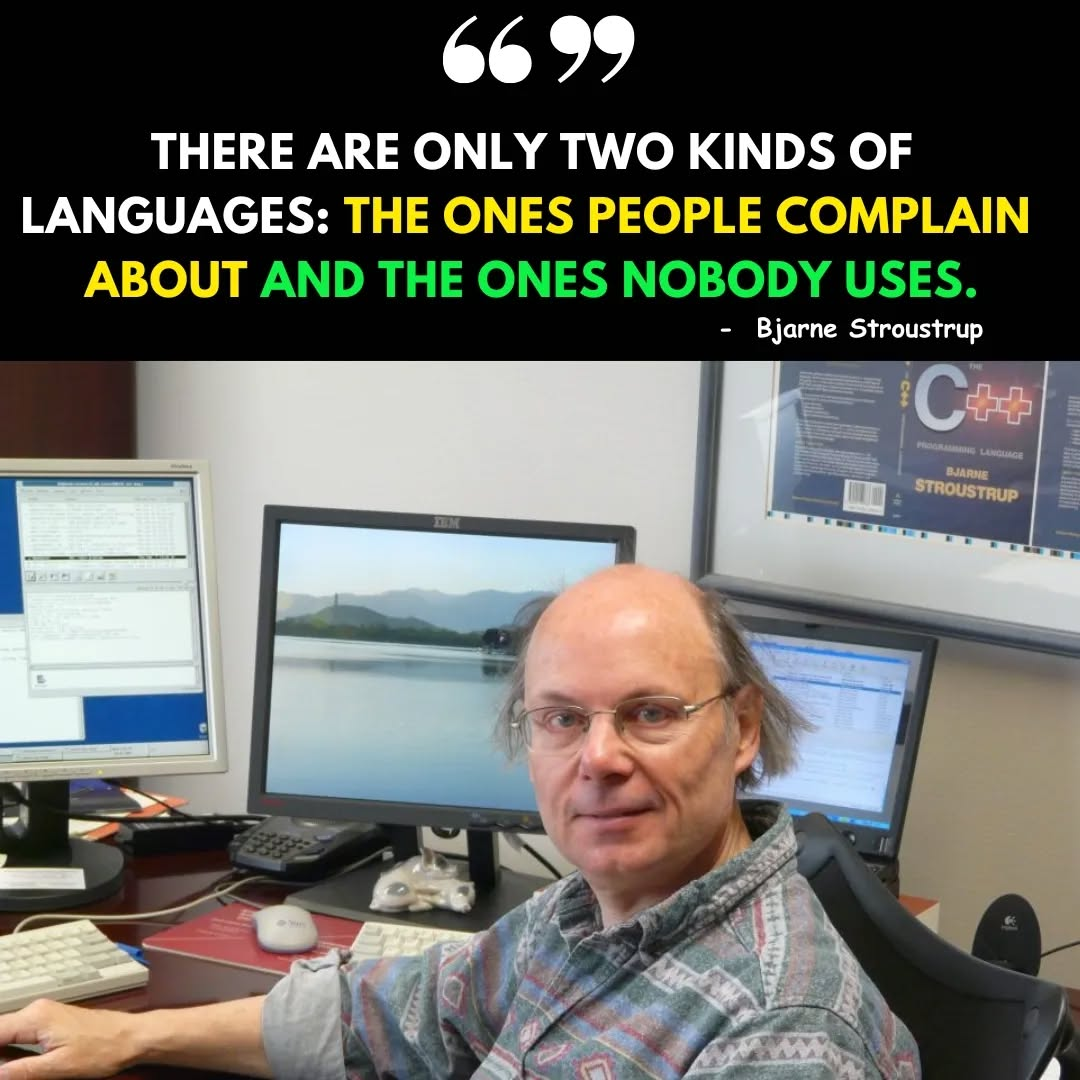
\includegraphics[width=0.2\textwidth]{images/cpp.png} &
        % \includegraphics[width=0.2\textwidth]{images/java.png} \\
        Smalltalk & C++ & Java
    \end{tabular}
\end{center}
\end{frame}

\section{The Eternal Battle: Bugs, Debugging, and Testing}

\begin{frame}{1947: The First "Computer Bug"}
\begin{columns}
    \begin{column}{0.5\textwidth}
        \begin{itemize}
            \item \textbf{September 9, 1947}: Operators of the Harvard Mark II computer found a moth trapped in a relay.
            \item The term "bug" had been used in engineering before, but this incident popularized it in computing.
            \item The moth was taped into the logbook with the note: "First actual case of bug being found."
            \item \textbf{Debugging} literally started as removing insects from hardware.
        \end{itemize}
    \end{column}
    \begin{column}{0.5\textwidth}
        % 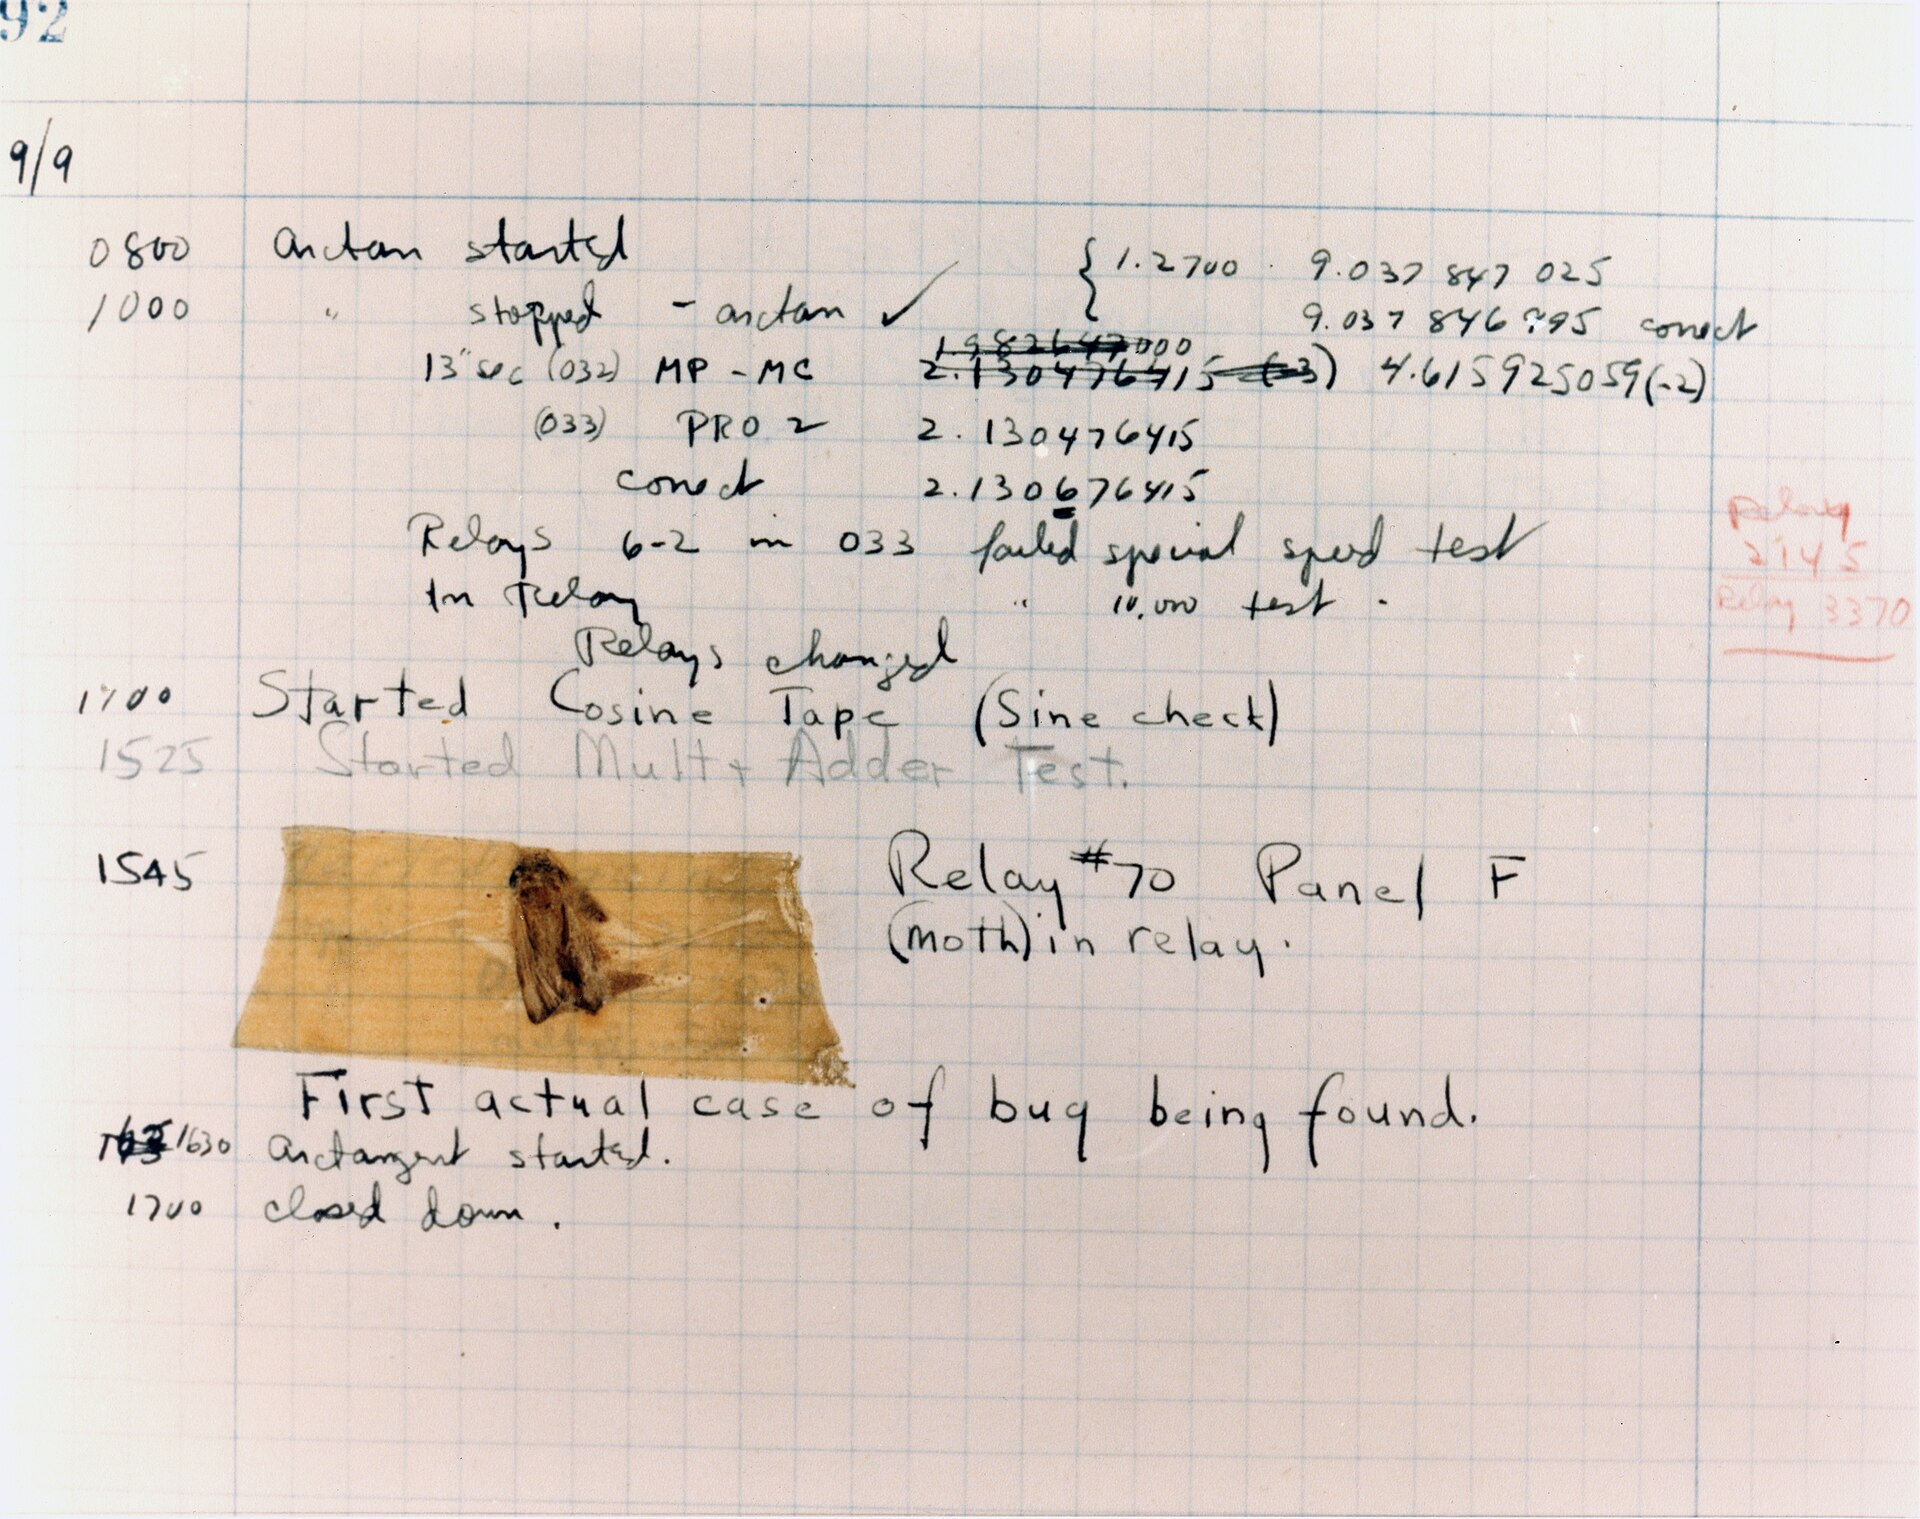
\includegraphics[width=0.9\textwidth]{images/first-computer-bug.jpg}
        \\\scriptsize{The first computer "bug" from the Harvard Mark II log book.}
    \end{column}
\end{columns}
\begin{block}{}
Early "debugging" was a physical, hardware-centric activity.
\end{block}
\end{frame}

\begin{frame}{1950s-1960s: The Dawn of Software Debugging}
\begin{itemize}
    \item \textbf{Print Statement Debugging}: The simplest and most enduring method. Programmers inserted print statements to trace program execution and variable states.
    \item \textbf{Core Dumps}: Analyzing the contents of memory after a program crash. A low-level, complex, but powerful technique.
    \item \textbf{Ad-hoc Testing}: Testing was manual, informal, and often performed by the developers themselves near the end of the project.
    \item \textbf{The Challenge}: As software grew in complexity, these methods became insufficient. The "software crisis" was, in part, a crisis of quality and reliability.
\end{itemize}
\begin{center}
    \texttt{printf("Got here! Value of x = \%d \textbackslash n", x);} % Example of a print statement
\end{center}
\end{frame}

\begin{frame}{1970s-1980s: Formalizing Testing and Tools}
\begin{columns}
    \begin{column}{0.6\textwidth}
        \textbf{The Rise of Testing Theory}
        \begin{itemize}
            \item \textbf{Black-box vs. White-box Testing}: Distinguishing between testing functionality (black-box) and testing internal structures (white-box).
            \item \textbf{Levels of Testing}: Unit, Integration, System, and Acceptance testing became standard concepts.
            \item \textbf{Static Analysis}: Compilers began to include more sophisticated warnings for potential code issues.
        \end{itemize}
        \textbf{The First Debugging Tools}
        \begin{itemize}
            \item \textbf{Symbolic Debuggers} (e.g., gdb): Allowed programmers to interact with a running program, set breakpoints, and inspect variables symbolically.
            \item This was a monumental leap from raw core dumps.
        \end{itemize}
    \end{column}
    \begin{column}{0.4\textwidth}
        % \includegraphics[width=0.8\textwidth]{images/gdb-screenshot.png}
        \\\scriptsize{Early GNU Debugger (GDB) interface.}
    \end{column}
\end{columns}
\end{frame}

\begin{frame}{1990s: Automation and Process Integration}
\begin{itemize}
    \item \textbf{Automated Regression Testing}: Tools like JUnit (1997) for Java, created by Kent Beck and Erich Gamma, revolutionized testing.
    \begin{itemize}
        \item Tests could be run automatically and frequently.
        \item Provided a safety net for refactoring and adding new features.
        \item Embodied the \textbf{Test-Driven Development (TDD)} philosophy.
    \end{itemize}
    \item \textbf{Testing Becomes a Discipline}: The role of \textbf{Quality Assurance (QA) Engineer} became specialized.
    \item \textbf{Continuous Integration (CI)}: Tools like CruiseControl automated the process of building and testing software after every change, catching integration bugs early.
\end{itemize}
\begin{center}
    % \includegraphics[width=0.7\textwidth]{images/junit-logo.png}
\end{center}
\end{frame}

\begin{frame}{2000s-2010s: Scaling and Shifting Quality Left}
\begin{columns}
    \begin{column}{0.6\textwidth}
        \textbf{Paradigm Shifts}
        \begin{itemize}
            \item \textbf{Shift-Left Testing}: The idea of testing earlier in the development lifecycle, involving QA and writing tests during development, not after.
            \item \textbf{Test Automation Pyramid}: A strategy for a balanced test suite: many fast, cheap Unit tests; fewer Integration tests; even fewer UI tests.
            \item \textbf{DevOps and Quality}: With rapid deployments, automated testing became non-negotiable. Quality is everyone's responsibility.
        \end{itemize}
        \textbf{New Frontiers}
        \begin{itemize}
            \item \textbf{Selenium}: Automated web browser testing.
            \item \textbf{Chaos Engineering}: Deliberately injecting failures into systems (e.g., Netflix's Chaos Monkey) to build resilience.
        \end{itemize}
    \end{column}
    \begin{column}{0.4\textwidth}
        % 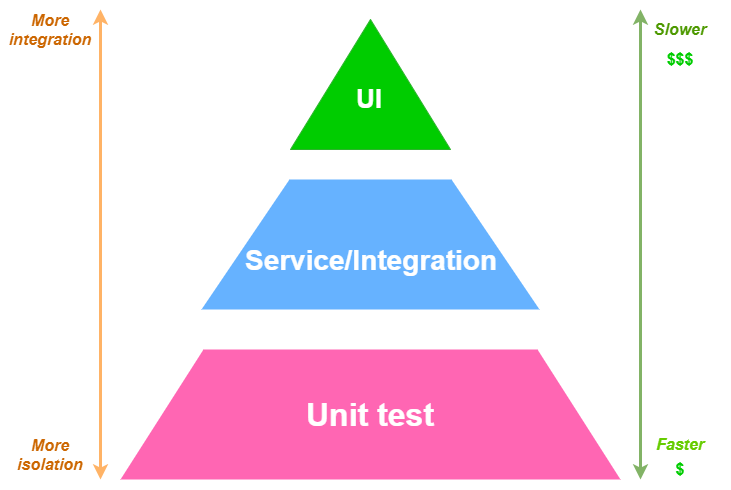
\includegraphics[width=\textwidth]{images/test-pyramid.png}
        \\\scriptsize{The Test Automation Pyramid.}
    \end{column}
\end{columns}
\end{frame}

\begin{frame}{2020s: The AI-Powered Future of Debugging}
\begin{itemize}
    \item \textbf{AI-Assisted Testing}:
    \begin{itemize}
        \item AI generates test cases, predicts flaky tests, and optimizes test suites.
        \item Tools can automatically detect visual regressions in UI.
    \end{itemize}
    \item \textbf{Intelligent Fault Localization}:
    \begin{itemize}
        \item AI analyzes code, execution traces, and bug reports to suggest the most likely lines of code causing a failure.
        \item \textbf{Example}: A tool like \textbf{Amazon CodeGuru} or \textbf{OpenAI's Debugger} can point directly to the suspicious code.
    \end{itemize}
    \item \textbf{Automated Program Repair}:
    \begin{itemize}
        \item LLMs can not only find bugs but also suggest and even generate fixes.
        \item \textbf{Example}: GitHub Copilot Chat can explain a bug and propose a patch.
    \end{itemize}
    \item \textbf{Observability}: The evolution beyond monitoring. Using logs, metrics, and traces (the three pillars) to understand the internal state of a system by its external outputs, making debugging in production much more effective.
\end{itemize}
\end{frame}

\begin{frame}{The Evolution of Debugging at a Glance}
\begin{center}
    \begin{tabular}{|l|l|l|l|}
    \hline
    \textbf{Era} & \textbf{Primary Method} & \textbf{Testing Focus} & \textbf{Key Innovation} \\
    \hline
    1940s-50s   & Physical Inspection & Ad-hoc & The Term "Bug" \\
    \hline
    1960s-70s   & Print Statements & Manual, Late & Symbolic Debuggers \\
    \hline
    1980s-90s   & Interactive Debuggers (gdb) & Formalized Test Levels & Automated Unit Testing (JUnit) \\
    \hline
    2000s-10s   & CI/CD Integrated Tools & Shift-Left, Automation & Test Pyramid, Chaos Engineering \\
    \hline
    2020s+      & AI-Powered Analysis & AI-Generated Tests & Intelligent Fault Localization \& Repair \\
    \hline
    \end{tabular}
\end{center}
\vspace{1em}
\begin{block}{The Unchanging Goal}
To move from \alert{reactive} bug-fixing to \alert{proactive} bug-prevention, and to reduce the time between discovering a failure and fixing it from months to minutes.
\end{block}
\end{frame}
\section{Modern Era}

\begin{frame}{2000s: Agile and DevOps}
\begin{columns}
    \begin{column}{0.6\textwidth}
        \begin{itemize}
            \item \textbf{Agile Manifesto} (2001)
            \item Emphasis on iterative development and customer collaboration
            \item \textbf{DevOps movement} (late 2000s)
            \item Bridging development and operations
            \item Continuous Integration/Continuous Deployment
            \item Infrastructure as Code
        \end{itemize}
    \end{column}
    \begin{column}{0.4\textwidth}
        % Add appropriate image
        % \includegraphics[width=\textwidth]{images/agile-devops.png}
    \end{column}
\end{columns}
\end{frame}

\begin{frame}{2010s: AIOps and Cloud Native}
\begin{itemize}
    \item \textbf{AIOps}: Applying AI to operations
    \begin{itemize}
        \item Automated monitoring and incident response
        \item Predictive analytics for system performance
        \item Anomaly detection and root cause analysis
    \end{itemize}
    \item \textbf{Cloud Native Development}
    \begin{itemize}
        \item Microservices architecture
        \item Containerization (Docker, Kubernetes)
        \item Serverless computing
    \end{itemize}
\end{itemize}
\begin{center}
    % Add appropriate image
    % \includegraphics[width=0.6\textwidth]{images/aiops-cloud.png}
\end{center}
\end{frame}

\section{LLM Era}

\begin{frame}{2020s: The LLM Revolution}
\begin{columns}
    \begin{column}{0.6\textwidth}
        \begin{itemize}
            \item \textbf{Large Language Models transform software engineering}
            \item GitHub Copilot (2021) and similar tools
            \item AI-assisted code generation and review
            \item Automated testing and documentation
            \item Shift in developer roles and skills
        \end{itemize}
    \end{column}
    \begin{column}{0.4\textwidth}
        % Add appropriate image
        % \includegraphics[width=\textwidth]{images/llm-coding.png}
    \end{column}
\end{columns}
\end{frame}

\begin{frame}{LLM Impact on Software Engineering}
\begin{itemize}
    \item \textbf{Code Generation}: From autocomplete to entire function generation
    \item \textbf{Debugging Assistance}: AI-powered bug detection and fixes
    \item \textbf{Documentation}: Automated documentation generation
    \item \textbf{Code Review}: AI-assisted quality assurance
    \item \textbf{Testing}: Intelligent test case generation
\end{itemize}
\begin{block}{Future Directions}
\begin{itemize}
    \item AI pair programmers becoming standard
    \item New programming paradigms emerging
    \item Focus shifting to prompt engineering and AI supervision
\end{itemize}
\end{block}
\end{frame}

\section{Conclusion}

\begin{frame}{Software Engineering Evolution Timeline}
\begin{center}
    % Add timeline image
    % 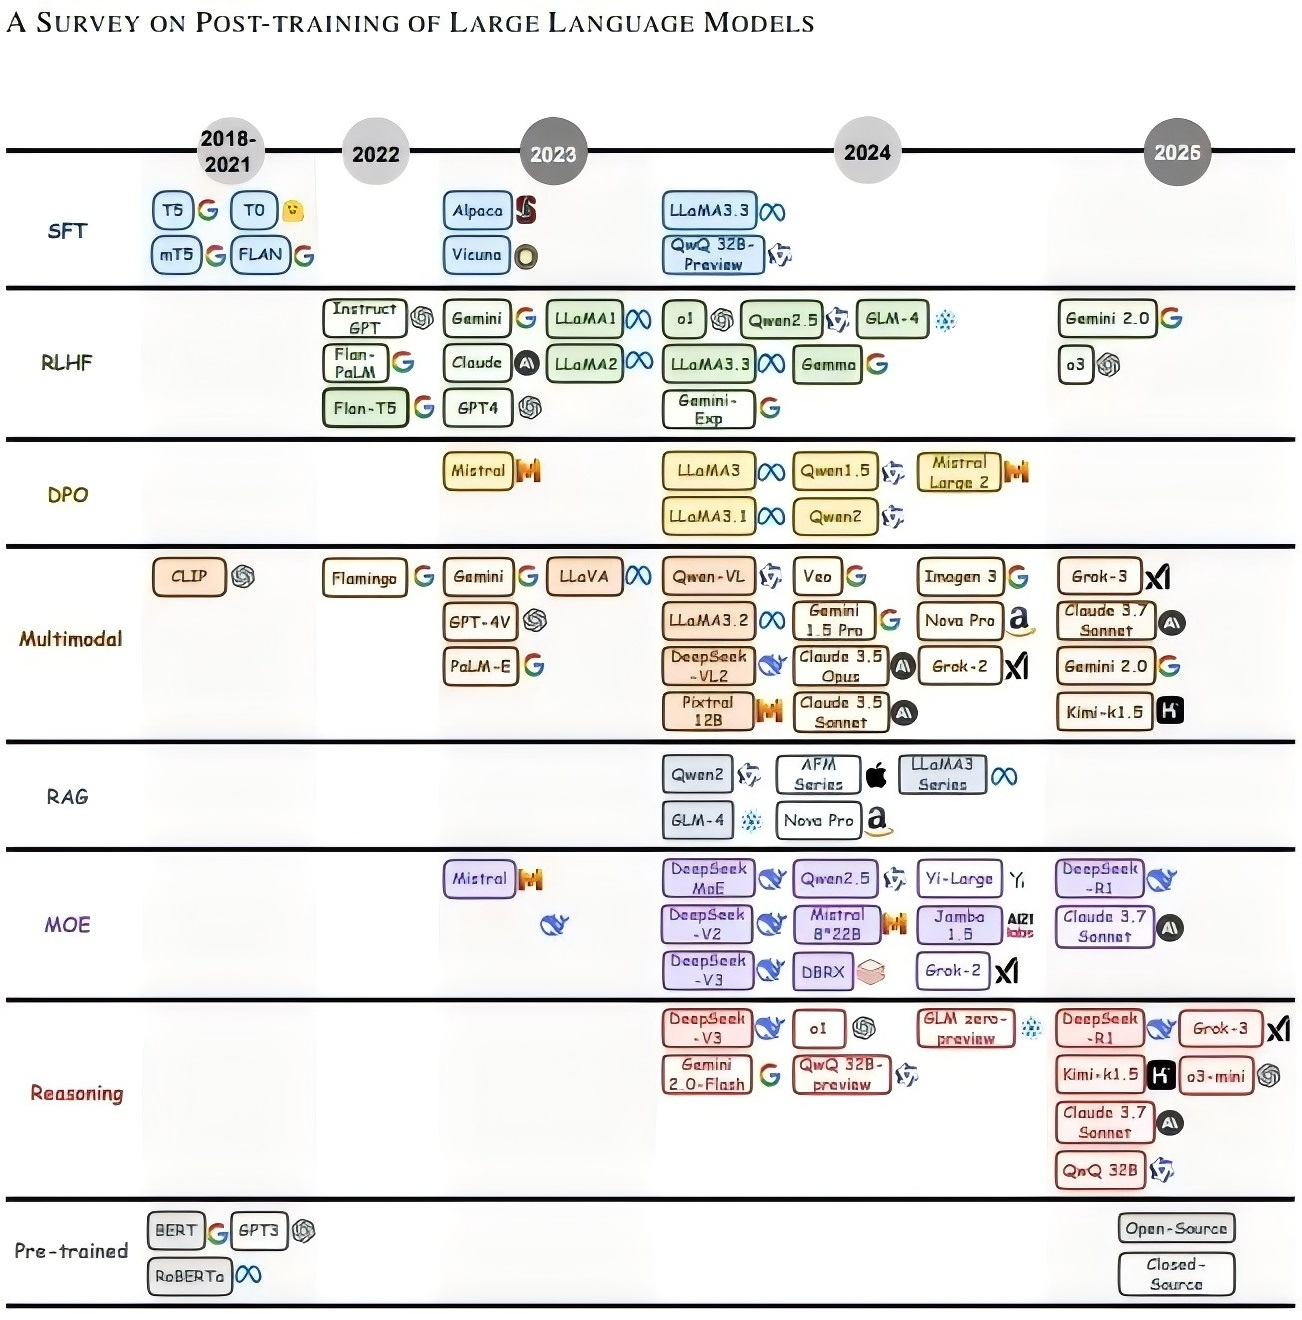
\includegraphics[width=0.9\textwidth]{images/timeline.png}
    \textbf{Visual Timeline Here}\\
    (1968 NATO → 1975 Man-Month → 1984 Trusting Trust → 1990s OSS/OOP → 2000s Agile/DevOps → 2010s Cloud → 2020s LLM)
\end{center}
\end{frame}

\begin{frame}{Looking Forward}
\begin{itemize}
    \item Continuous evolution from disciplined engineering to AI augmentation
    \item Increasing emphasis on automation and intelligence
    \item Software engineering becoming more accessible
    \item New challenges in ethics, security, and quality assurance
    \item The human element remains crucial in system design and oversight
\end{itemize}
\begin{center}
    \textbf{The journey continues...}
\end{center}
\end{frame}

\begin{frame}{References}
\begin{thebibliography}{10}
\bibitem{nato1968} NATO Software Engineering Conference (1968)
\bibitem{dijkstra1968} Dijkstra, E. W. (1968). "Go To Statement Considered Harmful"
\bibitem{brooks1975} Brooks, F. P. (1975). \textit{The Mythical Man-Month}. Addison-Wesley. % Added reference
\bibitem{thompson1984} Thompson, K. (1984). "Reflections on Trusting Trust"
\bibitem{stallman1983} Stallman, R. (1983). GNU Manifesto
\bibitem{beck2001} Beck, K. (2001). Agile Manifesto
\bibitem{llm2023} Chen, M. et al. (2023). "Evaluating Large Language Models Trained on Code"
\end{thebibliography}
\end{frame}

\end{document}
